\renewcommand{\thefigure}{S\arabic{figure}}
\renewcommand{\thetable}{S\arabic{table}}
\setcounter{figure}{0}
\setcounter{table}{0}

\begin{figure}
\centering
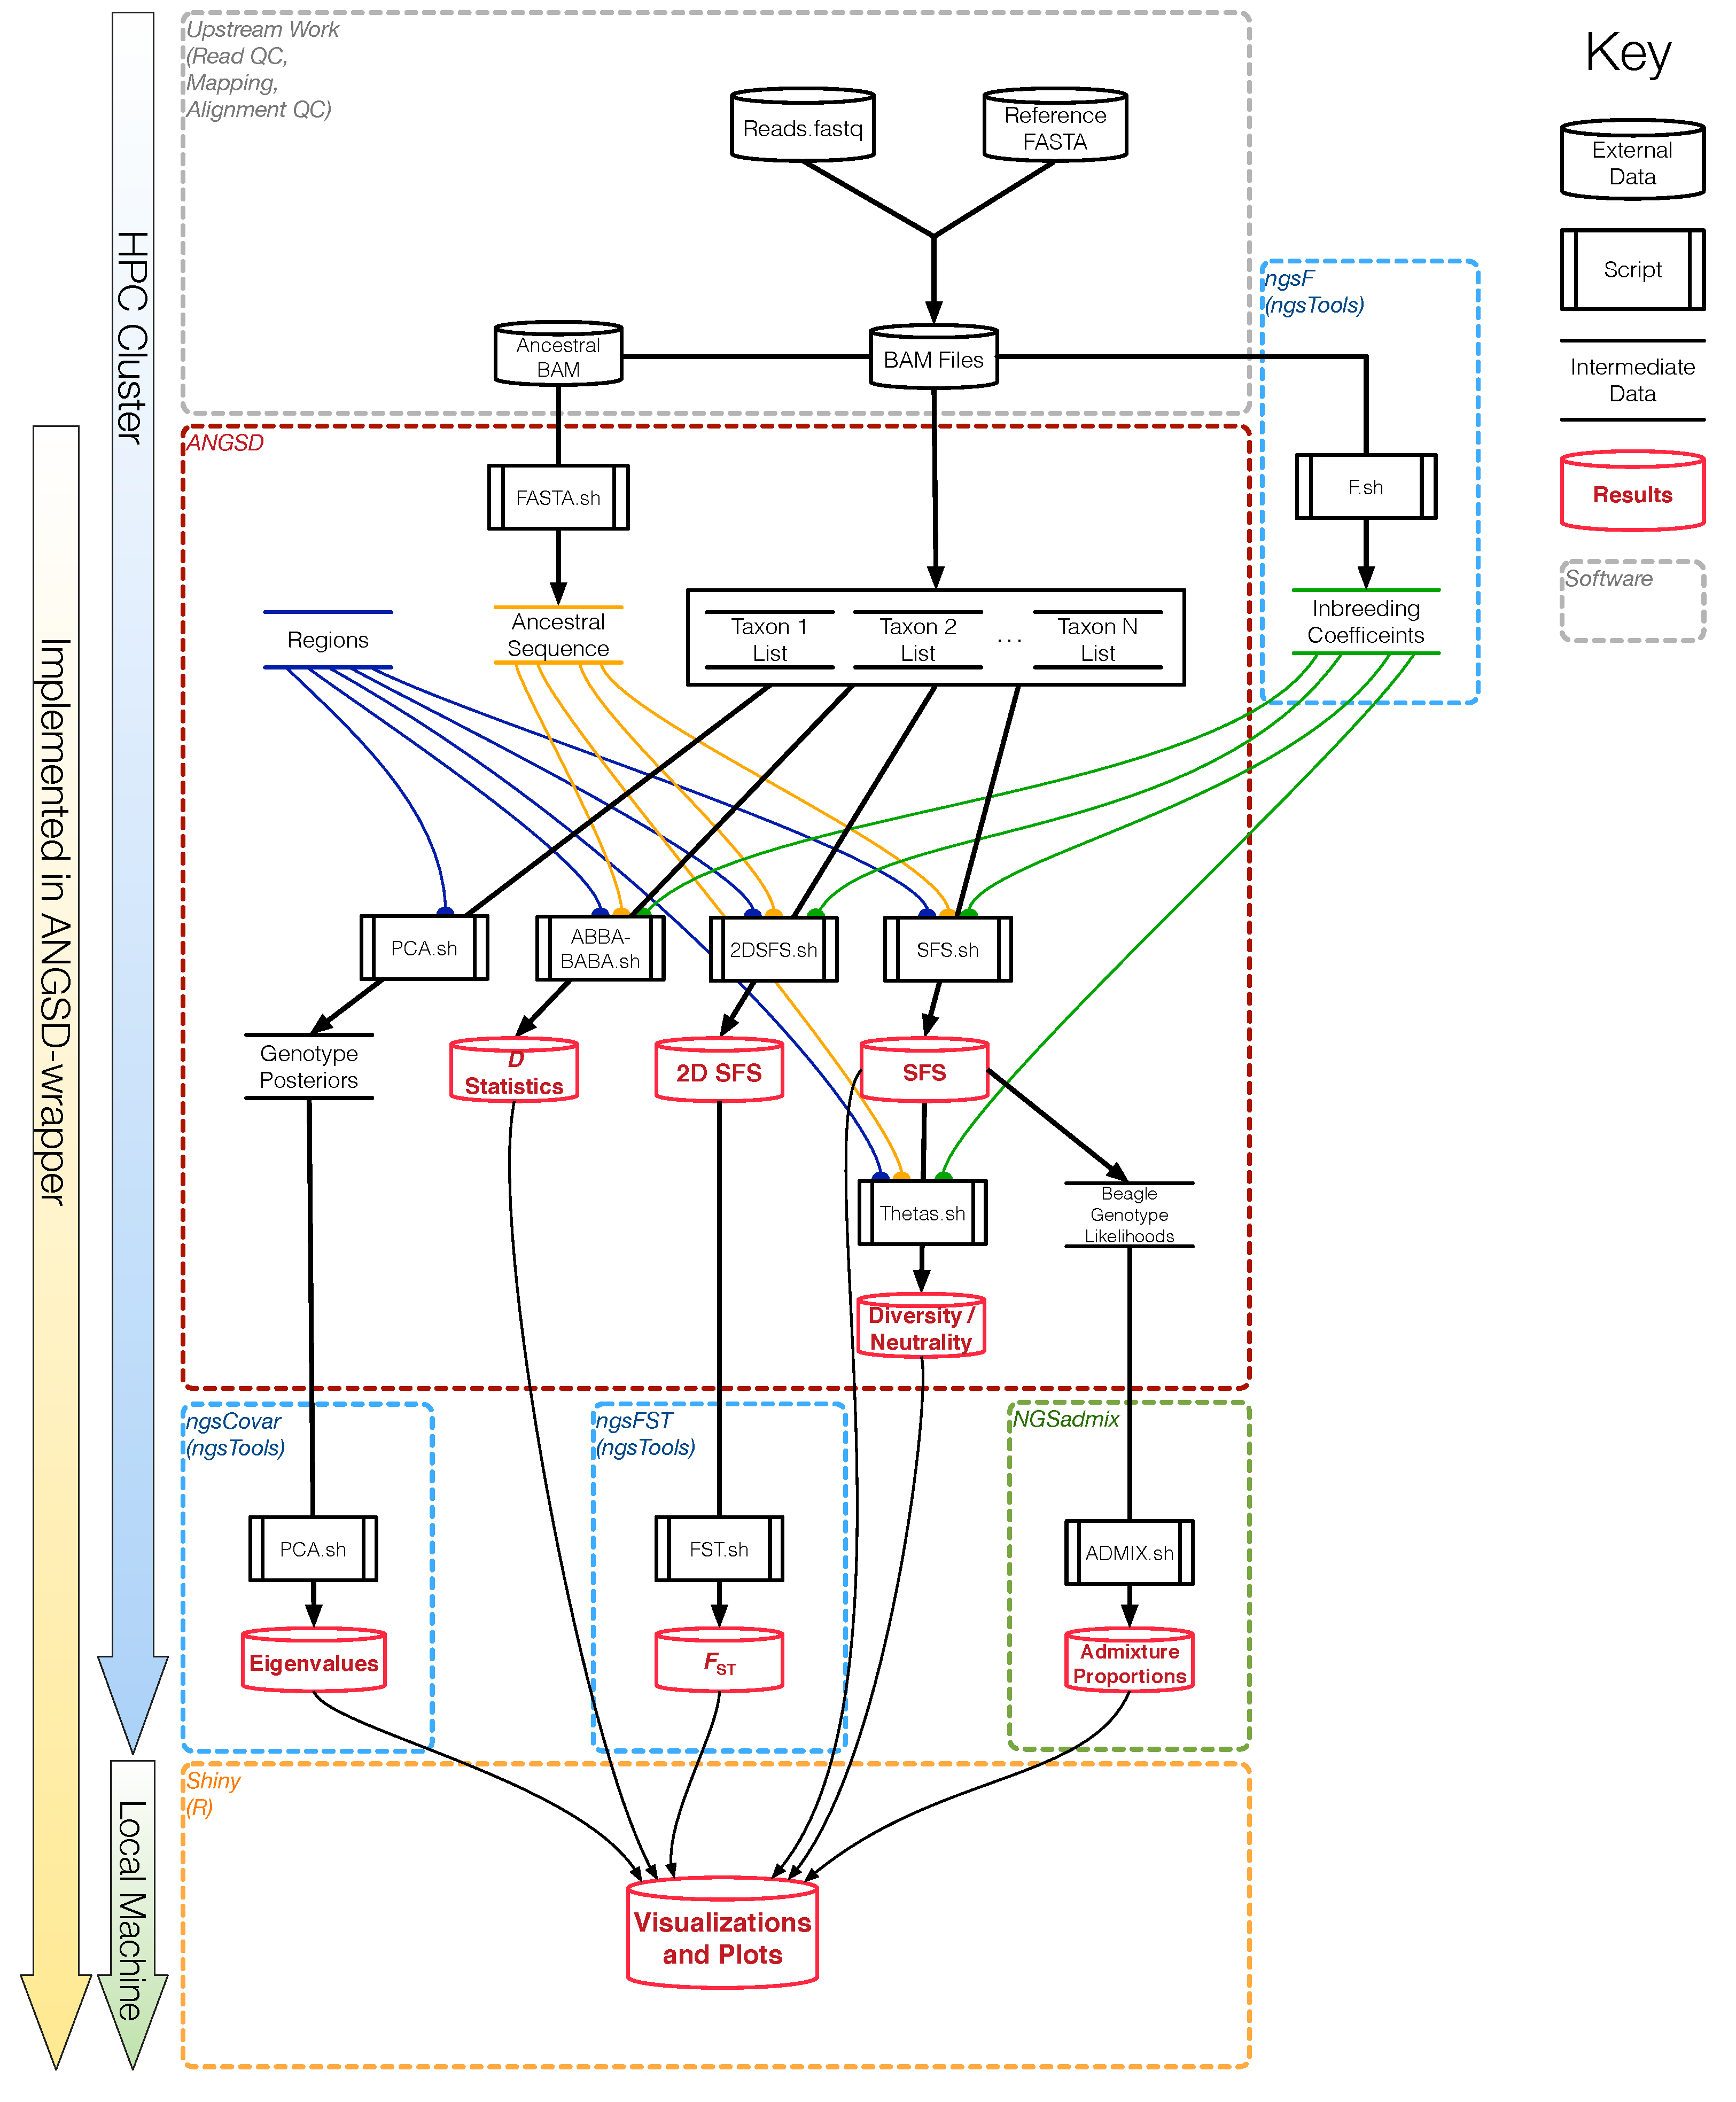
\includegraphics[width=\linewidth]{figures/Wiki_Workflow.pdf}
\caption{Workflow diagram for all methods available in ANGSD-wrapper.}
\label{fig:supp2}
\end{figure}

\begin{figure}
\centering
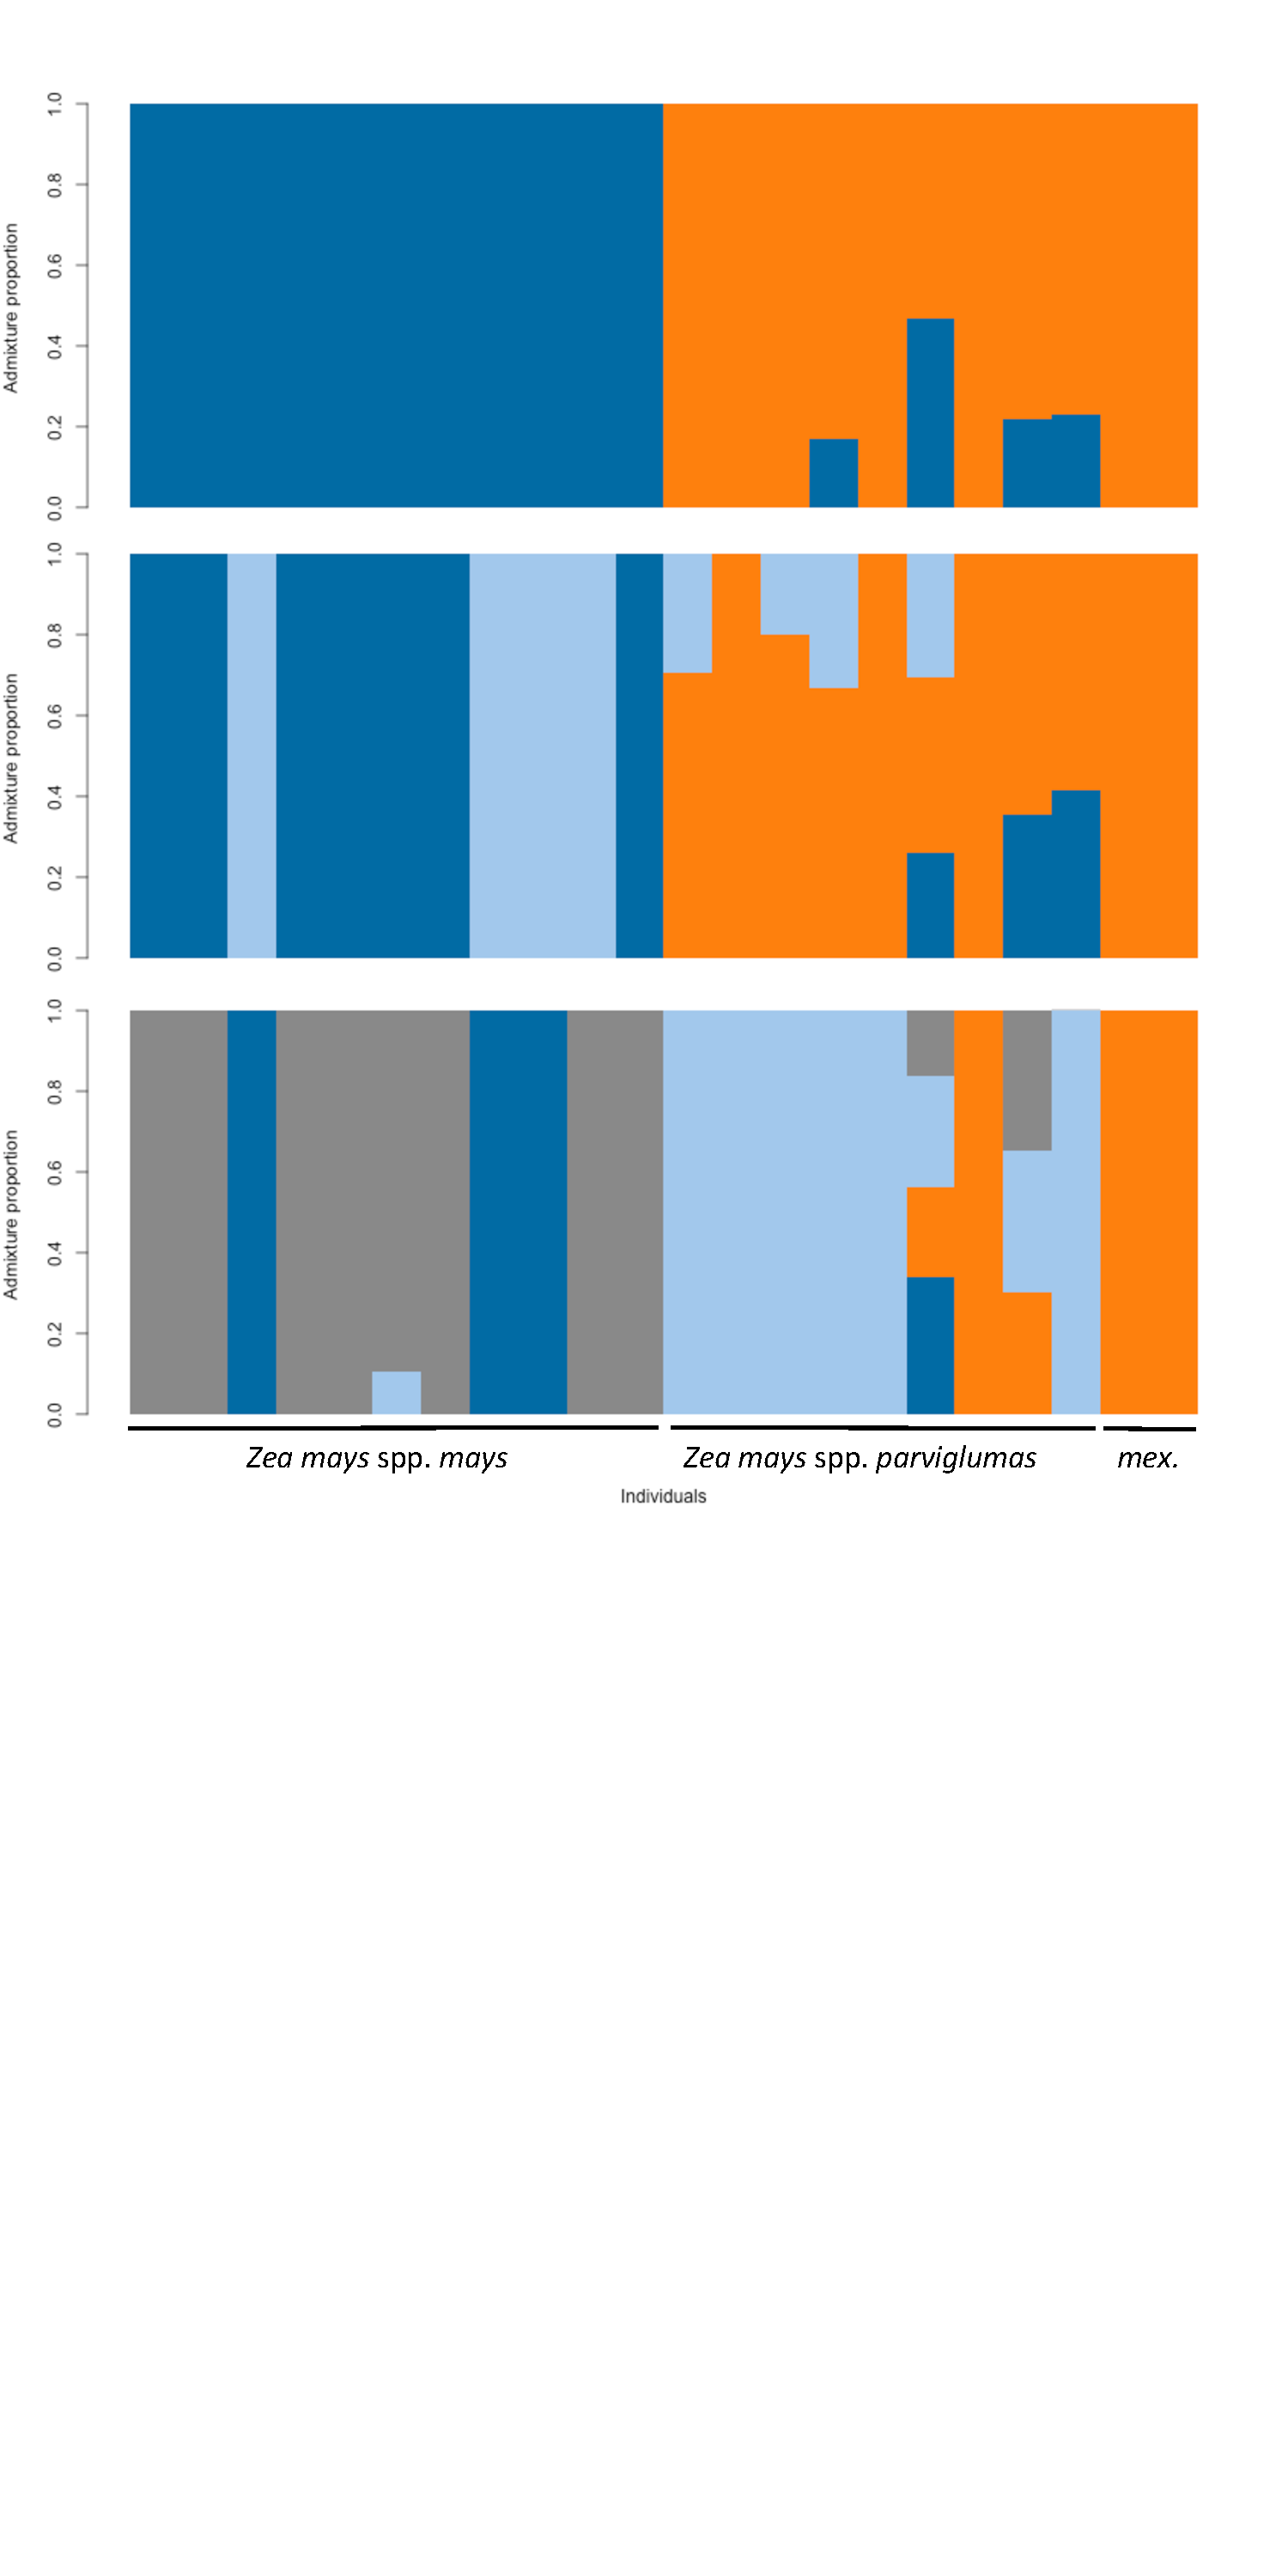
\includegraphics[width=\linewidth]{figures/admixture.pdf}
\caption{Admixture analysis for K=2 (top), K=3 (middle), and K=4 (bottom).}
\label{fig:suppadmix}
\end{figure}

\begin{table}
\begin{center}
	\begin{tabular} { | p{5cm} | p{5cm} | }
	\hline
	\textbf{Sample} & \textbf{Mean Depth} \\ \hline \hline
	BKN009 & 7.00194 \\ \hline
	BKN011 & 6.9777 \\ \hline
	BKN014 & 6.78829 \\ \hline
	BKN015 & 3.739 \\ \hline
	BKN019 & 3.71944 \\ \hline
	BKN022 & 3.71268 \\ \hline
	BKN025 & 3.53799 \\ \hline
	BKN026 & 3.91798 \\ \hline
	BKN027 & 7.05576 \\ \hline
	BKN033 & 3.85336 \\ \hline
	BKN035 & 3.74839 \\ \hline
	TIL01 & 3.60133 \\ \hline
	TIL03 & 4.07518 \\ \hline
	TIL04 & 6.09163 \\ \hline
	TIL07 & 5.11419 \\ \hline
	TIL09 & 5.29004 \\ \hline
	TIL11 & 3.15477 \\ \hline
	TIL15 & 6.87873 \\ \hline
	TIL16 & 2.67186 \\ \hline
	TIL17 & 2.61892 \\ \hline
	TIL08 & 6.09453 \\ \hline
	TIL25 & 13.1566 \\ \hline
	\end{tabular}
	\caption{Table of samples used in analysis with mean depth over the region 15000000-25000000 on chromosome 10}
	\label{tab:samples}
	\end{center}
\end{table}